\mcchap{Design e sviluppo della soluzione}{cap:designSviluppo}

\section{Origine dei dati}
La principale fonte di dati riguardanti la diffusione della pandemia da COVID-19 in Italia è il Dipartimento della Protezione Civile, che giornalmente a partire dal 24 febbraio pubblica i relativi dati sul repository Github\cite{repository}.

Alcuni dati resi disponibili sul repository sono i seguenti:
\begin{itemize}
    \item Ricoverati con sintomi: numero di soggetti ricoverati non in terapia intensiva.
    \item Terapia intensiva: Numero di soggetti ricoverati in terapia intensiva.
    \item Totale ospedalizzati: Totale dei soggetti ricoverati in ospedale.
    \item Isolamento domiciliare: Soggetti ricoverati presso la propria abitazione.
    \item Deceduti: Persone decedute positive al virus.
    \item Tamponi: numero di tamponi effettuati (antigenici + molecolari)
\end{itemize}


\begin{figure}[htp]
    \centering
    
\includegraphics[width=5cm]{logo_dpc}
    \caption{Logo del Dipartimento della Protezione Civile}
\end{figure}


\section{Tecnologie utilizzate}
In questa sezione verranno elencate alcune delle tecnologie utilizzate per lo sviluppo del progetto.

\subsection{Python}
Python è un linguaggio di programmazione dinamico orientato agli oggetti utilizzabile per molti tipi di sviluppo software, è completamente gratuito ed è utilizzabile senza restrizioni di copyright.\\
Python è un linguaggio portabile sviluppato in ANSI C, è caratterizzato da una sintassi essenziale, ma consente lo sviluppo di applicazioni molto complesse.\\
È multipiattaforma e quindi utilizzabile su diversi  sistemi operativi quali Windows, MacOS e GNU/Linux.
Offre un forte supporto all'integrazione con altri linguaggi e programmi, dispone di una estesa libreria standard e funzioni matematiche integrate, che semplificano il calcolo dei problemi matematici e l'esecuzione dell'analisi dei dati.
\noindent Per lo sviluppo del progetto è stato utilizzato interamente il linguaggio Python versione 3.8.
\begin{figure}[htp]
    \centering
    
\includegraphics[width=4cm]{python_logo}
    \caption{Logo di Python}
\end{figure}

\subsection{Plotly}

Plotly è una libreria Python open source  per la creazione di grafici interattivi, supporta oltre 40 tipologie diverse di grafici che consentono l’applicazione in vari campi scientifici, tra i quali la statistica, la finanza, e la geografia.
Plotly basa il suo funzionamento sulla libreria Javascript plotly.js, che permette agli utenti Python di realizzare stupende applicazioni di visualizzazione dati interattive, che si possono mostrare in un file HTML indipendente, in un Notebook Jupyter\footnotemark, oppure all’interno di una applicazione web utilizzando Dash.
\footnotetext{Jupyter Notebook è un'applicazione web open source che consente di creare e condividere documenti che contengono codice Python eseguibile in tempo reale, equazioni, visualizzazioni.}

\begin{figure}[htp]
    \centering
    
\includegraphics[width=4cm]{plotly_logo}
    \caption{Logo di Plotly}
\end{figure}

\subsection{Pandas}
Pandas è una libreria Python open source, adatta per l’analisi e la manipolazione di dati in formato sequenziale o tabellare.
Pandas consente il Caricamento e il salvataggio di formati standard per dati tabellari, come CSV (Comma-separated Values).
Una delle strutture dati utilizzate da Pandas prende il nome di DataFrame, una struttura dati bi-dimensionale, con dimensione variabile che può contenere dati eterogenei.
\begin{figure}[htp]
    \centering
    
\includegraphics[width=4cm]{pandas_logo}
    \caption{Logo di Pandas}
\end{figure}

\subsection{Dash}
Dash è un framework Python ideato per la costruzione di applicazioni web di analytics, si appoggia a Flask\footnote{Flask è un framework leggero sviluppato da Armin Ronacher per applicazioni web WSGI
(Web Server Gateway Interface)}, Plotly.js e react.js\footnotemark.
Dash è ideale per la costruzione di applicazioni di visualizzazione dati molto personalizzabili, usando soltanto il linguaggio Python. 
È particolarmente indicato per chiunque lavori con i dati in Python.
Attraverso l’utilizzo di semplici pattern, Dash semplifica notevolmente la costruzione di applicazioni basate su web, come nel caso della dashboard, in quanto non è necessario conoscere approfonditamente le tecnologie e i protocolli che ne determinano il funzionamento.
\footnotetext{React è una libreria JavaScript per la creazione di interfacce utente.}

\begin{figure}[htp]
    \centering
    
\includegraphics[width=4cm]{dash_logo}
    \caption{Logo di Dash}
\end{figure}


\subsection{Github}
\noindent GitHub è un servizio web basato su cloud che aiuta gli sviluppatori ad archiviare e gestire il loro codice e a tracciare e controllare le modifiche.

\noindent Git è un sistema che consente il controllo delle versioni e permette a più sviluppatori di collaborare allo stesso progetto contemporaneamente.
\noindent In sostanza Github, semplifica l’utilizzo del software a riga di comando Git per il controllo delle versioni e la collaborazione.


\begin{figure}[htp]
    \centering
    
\includegraphics[width=3cm]{github_logo}
    \caption{Logo di Github}
\end{figure}

\subsection{Docker}
\noindent Docker è un progetto open source nato con lo scopo di automatizzare la distribuzione di applicazioni sotto forma di “contenitori” detti container.
I container hanno al loro interno tutto il necessario per la corretta esecuzione dell’applicazione, incluse librerie, strumenti di sistema, codice e runtime.

\begin{figure}[htp]
    \centering
    
\includegraphics[width=4cm]{docker_logo}
    \caption{Logo di Docker}
\end{figure}

\noindent Un container è basato su un’immagine che rappresenta tutto il suo contenuto e definisce quale applicativo sarà eseguito al suo interno. 
Per il progetto è stato scelto Docker in quanto consente di isolare una dashboard dalle altre e pertanto semplifica il processo di distribuzione e aggiornamento.

\section{Lo sviluppo}
Lo sviluppo del progetto è iniziato partendo dai dati contenuti in un foglio di calcolo Excel fornito dal professore, dal quale sono state estrapolate le formule necessarie per l’elaborazione degli stessi atti alla costruzione della dashboard.

\subsection{Calcoli dei dati}
I calcoli vengono effettuati direttamente nella struttura DataFrame di Pandas
\begin{figure}[htp]
    \centering
    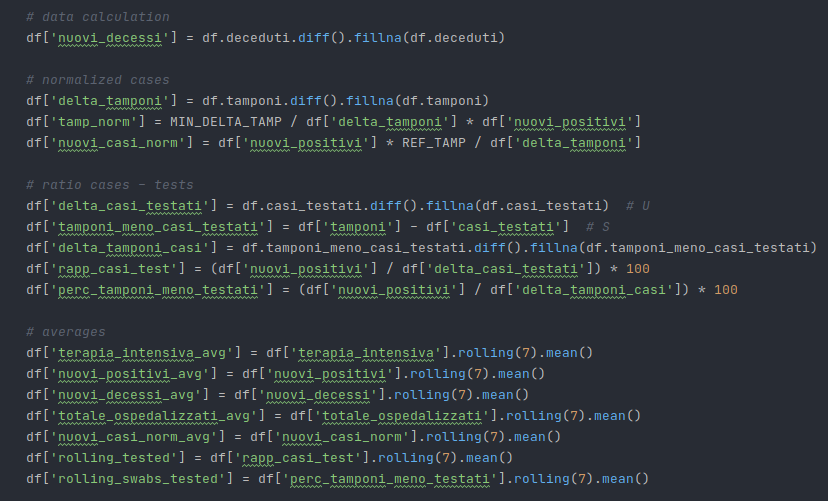
\includegraphics[width=10cm]{data_calculation}
    \caption{Codice Python per il calcolo dei dati}
\end{figure}

\subsection{Diagramma di attività}
Un diagramma di attività UML è un diagramma di flusso che rappresenta il flusso del programma da un'attività all'altra, da un punto iniziale (punto nero pieno) a un punto finale (punto nero cerchiato).
Nella figura \ref{fig:activity} è raffigurato il diagramma delle attività per la dashboard.
\begin{figure}[htp]
    \centering
    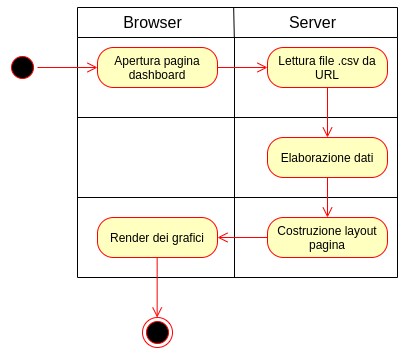
\includegraphics[width=10cm]{activity}
    \caption{Diagramma di attività}
    \label{fig:activity}
\end{figure}

\subsection{Organizzazione file}
Una applicazione Dash è composta essenzialmente da un singolo programma Python.
La cartella \emph{assets} contiene il file \emph{bootstrap.min.css}, una versione minimale del framework Bootstrap,\footnotemark questo assicura dei tempi di caricamento della pagina decisamente più rapidi.
Questa cartella contiene anche i loghi delle regioni, nella dashboard delle regioni (nella figura \ref{fig:tree_regioni}.
\footnotetext{Bootstrap è un framework CSS utilizzato per la semplificare la gestione dello stile della dashboard}

\begin{figure}
\centering
\begin{minipage}{.3\linewidth}
\dirtree{%
.1 italy.
.2 assets.
.3 bootstrap.min.css.
.2 dash\_italy.py.
}
\caption{Struttura file dashboard Italia}
\label{fig:tree_italia}
\end{minipage}\hfill
\begin{minipage}{.3\linewidth}
\dirtree{%
.1 lombardia.
.2 assets.
.3 bootstrap.min.css.
.2 dash\_lombardia.py.
}
\caption{Struttura file dashboard Lombardia}
\label{fig:tree_lombardia}
\end{minipage}
\end{figure}
% seconda figura
\begin{figure}
\centering
\begin{minipage}{.3\linewidth}
\dirtree{%
.1 regioni.
.2 assets.
.3 bootstrap.min.css.
.3 img.
.4 Abruzzo.png.
.4 Basilicata.png.
.4 Calabria.png.
.4 ....
.2 dash\_regioni.py.
}
\caption{Struttura file dashboard regioni}
\label{fig:tree_regioni}
\end{minipage}\hfill
\end{figure}

\section{Problemi riscontrati}
I dati forniti dal Dipartimento della Protezione Civile non sono esenti da errori, ciò può essere dovuto a errori di trascrizione oppure a causa di comunicazioni parziali o in ritardo dal parte delle regioni.
\noindent Alcune serie di dati, come ad esempio quelli cumulativi come guariti, deceduti, totale casi e tamponi, che dovrebbero essere strettamente crescenti, alcune volte non lo sono.

\subsection{Errore nei tamponi}
Il 17 dicembre 2020 è stato registrato un valore incorretto nel valore cumulativo dei tamponi, ciò ha causato un anomalia nel grafico dei casi normalizzati.\\
Per la correzione di questo problema è stato effettuato un intervento di pulizia del dato.
Il dato "incriminato" è stato sostituito con la media tra il giorno precedente e quella del giorno successivo.
\begin{figure}[htp]
    \centering
    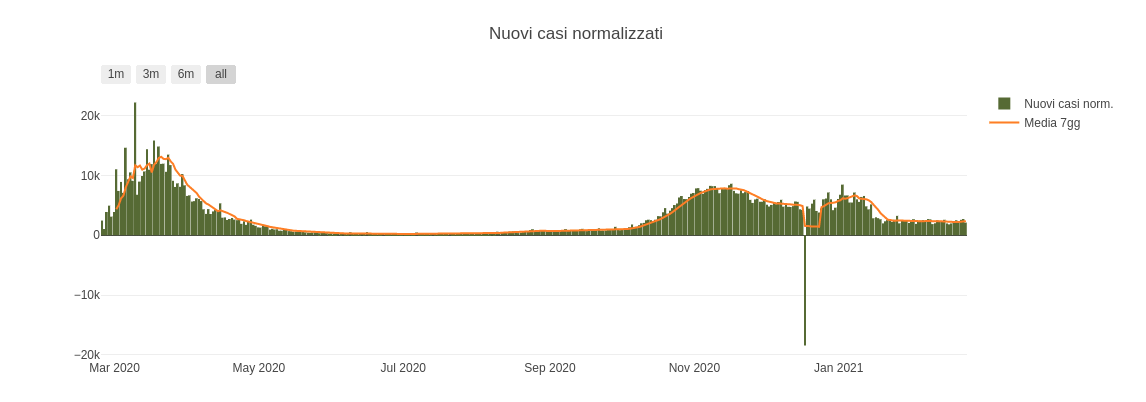
\includegraphics[width=14cm]{chart_problem}
    \caption{Problema causato dal valore incorretto dei tamponi}
\end{figure}


